\chapter{Method}
\label{chap:method}

\section{Problem Formulation}
\label{sec:formulation}
A run processes tasks $t_1,\dots,t_n$ ($n=101$) in a fixed order. Task $t_i$ has a requirement $r_i$ and hidden test cases $c_{i,1},\dots,c_{i,m_i}$. A generator $G$ with fixed parameters maps prompt $x_i$ to project $y_i=G(x_i)$, and evaluator $E$ assigns accuracy $a_i=E(y_i, c_{i,\cdot})\in[0,1]$ as defined in \Cref{chap:setup}. With No Memory, $x_i=r_i$. With memory,
\begin{equation}
x_i = r_i \oplus f(r_i, M_{i-1}), \qquad M_i = u\bigl(M_{i-1}, r_i, y_i, \tau_i, a_i\bigr),
\end{equation}
where $M_0=\emptyset$, $f$ selects and formats information from the memory available before task $t_i$, $\oplus$ appends it to the requirement, $\tau_i$ is the evaluator transcript, and $u$ updates the memory only after the task has been evaluated. Because $f$ reads only $M_{i-1}$, evaluation of $t_i$ cannot affect its own prompt. The generator, evaluator, and protocol are identical across arms. \Cref{alg:pipeline} and \Cref{fig:memflow} describe the final design (\Cref{sec:pipeline}); \Cref{sec:nm-failures} first presents the failures that motivated it.

\begin{algorithm}[ht]
\caption{Cross-task memory for one run (final version).}
\label{alg:pipeline}
\begin{algorithmic}[1]
\State $S_0=(M_0,F_0,C_0) \gets (\emptyset,\emptyset,\emptyset)$ \Comment{lessons, code facts, versioned code pool}
\For{$i = 1,\dots,n$}
  \State $L \gets \textsc{Checklist}(r_i)$ with at most three hard-match lessons from $M_{i-1}$
  \State $P \gets \textsc{SelectActive}(C_{i-1}, r_i)$ \Comment{$\le 3$ active entries}
  \State $x_i \gets r_i \oplus L \oplus P$; \quad $y_i \gets G(x_i)$; \quad $(a_i,\tau_i) \gets E(y_i)$
  \State $M_i \gets \textsc{Reflect}(M_{i-1}, r_i, y_i, \tau_i, a_i)$ \Comment{deduplicate; update utilities}
  \State $F_i \gets F_{i-1} \cup \textsc{StaticAnalyse}(y_i)$
  \State $C_i \gets \textsc{UpdatePool}(C_{i-1}, F_i, \{y_j : j\le i,\ a_j \ge 0.5\})$ \Comment{activate, verify, version}
\EndFor
\end{algorithmic}
\end{algorithm}

\noindent \textsc{StaticAnalyse} records undeclared imports, Vue functions used without import, and compile errors. \textsc{UpdatePool} is described in \Cref{sec:codepool}, while \Cref{tab:params} gives the fixed constants.

\begin{figure}[ht]
\centering
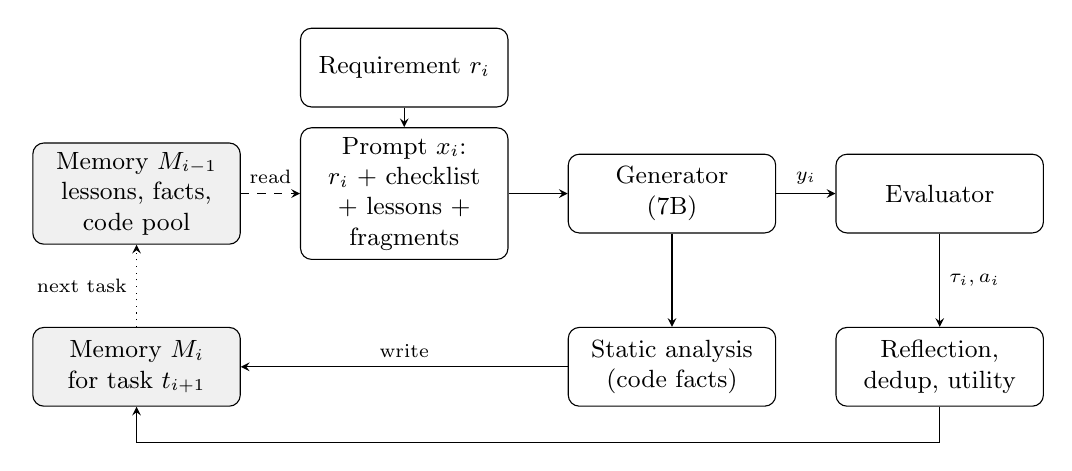
\begin{tikzpicture}[every node/.style={font=\small},
  box/.style={draw, rounded corners, align=center, minimum height=10mm, text width=2.4cm},
  mem/.style={draw, rounded corners, fill=gray!12, align=center, minimum height=10mm, text width=2.4cm}, >=stealth]
\node[mem] (M0) at (0,0) {Memory $M_{i-1}$\\lessons, facts,\\code pool};
\node[box] (req) at (3.4,1.6) {Requirement $r_i$};
\node[box] (pr) at (3.4,0) {Prompt $x_i$:\\$r_i$ + checklist\\+ lessons + fragments};
\node[box] (gen) at (6.8,0) {Generator\\(7B)};
\node[box] (ev) at (10.2,0) {Evaluator};
\node[box] (sa) at (6.8,-2.2) {Static analysis\\(code facts)};
\node[box] (ref) at (10.2,-2.2) {Reflection,\\dedup, utility};
\node[mem] (M1) at (0,-2.2) {Memory $M_i$\\for task $t_{i+1}$};
\draw[->, dashed] (M0) -- node[above,font=\scriptsize]{read} (pr);
\draw[->] (req) -- (pr);
\draw[->] (pr) -- (gen);
\draw[->] (gen) -- node[above,font=\scriptsize]{$y_i$} (ev);
\draw[->] (gen) -- (sa);
\draw[->] (ev) -- node[right,font=\scriptsize]{$\tau_i, a_i$} (ref);
\draw[->] (ref.south) -- ++(0,-0.45) -| (M1.south);
\draw[->] (sa) -- node[above,font=\scriptsize]{write} (M1);
\draw[->, dotted] (M1) -- node[left,font=\scriptsize]{next task} (M0);
\end{tikzpicture}
\caption[The memory flow of the final method.]{The memory flow of the final method. Dashed arrows read the memory built from earlier tasks; the lower row writes memory after evaluation. $r_i$: requirement; $y_i$: generated site; $\tau_i$: evaluator transcript; $a_i$: score; $M_{i-1}$, $M_i$: memory before and after $t_i$.}
\label{fig:memflow}
\end{figure}


\section{Starting Point: Why No Memory Fails}
\label{sec:nm-failures}
The initial analysis examined generated code rather than scores alone. Two observations shaped the later design.

\paragraph{Blank pages from basic errors.} Bolt.diy's Vue template declares only \texttt{vue} as a dependency, and WebGen-LM-7B did not edit \texttt{package.json} in any of the 81 inspected responses. When it imported \texttt{vue-router}, or used a Vue function such as \texttt{ref} without importing it, the site rendered as a blank page and all test cases failed. In an early Long Memory run, 26 of 74 tasks produced blank pages; 19 of those failures involved an undeclared \texttt{vue-router} import. In many cases, functional difficulty cannot be assessed because the site fails before any requested behaviour can be evaluated.

\paragraph{Text is not followed.} A targeted diagnostic, rather than a powered experiment, used nine tasks that had produced blank pages. Their original prompts were retained while one sentence was added in several forms: ``add vue-router to package.json'', ``do not use vue-router'', ``put pages in App.vue with \texttt{ref} and \texttt{v-if}'', or the same instruction at both the beginning and end of the prompt. No phrasing recovered more than one task out of three; each was tried on three of the nine tasks, and a task counted as recovered when the generated code imported no undeclared package and compiled. A ten-line code example implementing the same idea, tested on all nine tasks, recovered seven. The text variants and code example were evaluated on different task subsets, so this finding is suggestive rather than conclusive. It nevertheless indicated that code might be a more usable memory representation for this model, consistent with evidence that small models follow instructions less reliably~\cite{harada2025curse,li2025smallmodels}.

\section{Final Method}
\label{sec:pipeline}
For every task, the pipeline proceeds in the following order.
\begin{enumerate}
  \item \textbf{Build a requirement checklist.} The memory model divides the requirement into items (\Cref{sec:checklist}).
  \item \textbf{Retrieve lessons.} It also decomposes the requirement into no more than three functional \emph{aspects}, each defined by a feature, user trigger, expected state change, and domain-independent interaction pattern, plus appearance aspects. Functional lessons are retrieved by similarity and assessed as a hard match (the same trigger and state change), soft transfer (the same interaction type), or reject. Only hard matches are attached to checklist items. A small common pool contributes site-wide lessons containing a concrete code construct.
  \item \textbf{Select code.} At most three verified fragments are added when their trigger conditions hold (\Cref{sec:codepool}).
  \item \textbf{Generate and evaluate.} WebGen-LM-7B generates one project, which then undergoes the official functional and appearance evaluation.
  \item \textbf{Reflect and store.} The memory model reflects on the evaluated task. New lessons are deduplicated, utility estimates are updated, and code facts are recorded for the pool.
\end{enumerate}
The products of step 5 can influence only later tasks through steps 2 and 3. \Cref{fig:prompt} illustrates the resulting prompt. Under No Memory, the first requirement paragraph is the full prompt.

\begin{figure}[ht]
\begin{lstlisting}[basicstyle=\ttfamily\scriptsize]
Please implement an online trading website for bidding and trading. [...] Set the
background color to lemon chiffon and the component color to chocolate.

FEATURE CHECKLIST (the requirement above, item by item; build every item):
1. Please implement an online trading website for bidding and trading.
3. allowing users to browse trading opportunities,
   Note from earlier websites: For the trading opportunities: use `v-for` to
   display the list with current status.
[... items 2, 4-8 ...]

CODE FROM EARLIER WEBSITES THAT WORKED:
Component fails: ref() not imported. Earlier websites broke here (a component
calls ref() without importing it from 'vue' (that page fails when opened),
19 tasks). Code that works:
    import { ref, onMounted } from 'vue'
    const wheelRef = ref<HTMLElement | null>(null)
Vue compile error: v-model on prop. [...] (4 tasks). Code that works:
    <SearchBar :modelValue="searchQuery"
               @update:modelValue="emit('update:searchQuery', $event)" />
[... one more entry ...]

Build every checklist item; the notes only warn about mistakes earlier websites made.
\end{lstlisting}
\caption{The final method's prompt for task 000041 (seed 11), shortened: requirement, checklist with attached lessons, and verified code fragments.}
\label{fig:prompt}
\end{figure}

\subsection{Requirement Checklist}
\label{sec:checklist}
The original requirement remains at the beginning of the prompt and is explicitly binding. The checklist repeats each requested feature so that added memory does not displace a requirement from the model's attention~\cite{liu2024lost,wallace2024hierarchy}. Lessons are attached to the checklist item to which they apply, rather than presented as a separate list that could be mistaken for the task's complete scope.

\subsection{Code Pool}
\label{sec:codepool}
Detection for the code pool does not rely on an \gls{llm}.
\begin{itemize}
  \item \textbf{Problem facts.} After each task, static analysis records undeclared imports (\texttt{import:<package>}), Vue functions used without import (\texttt{vue-api}), and compile errors. Imports are checked against \texttt{package.json}. Vue-function use is detected when a function name is followed by \texttt{(} or \texttt{<} in a script that neither imports nor defines it. Each Vue \gls{sfc} is compiled with \texttt{@vue/compiler-sfc} in the same script-template combination used by Vite's Vue plugin, without type checking or bundling.
  \item \textbf{Trigger.} A problem key becomes active after appearing in two different tasks, following Metis's policy of promoting a procedure only after recurrence~\cite{dai2026metis}. Objectively detected whole-site failures, such as undeclared packages and compile errors, become active after one occurrence. Missing-import and compile-error entries apply to every Vue site. Other entries are used only when the memory model judges their condition to be present in the requirement.
  \item \textbf{Source.} Examples come from earlier websites in the same chain that score at least 0.5, compile, and contain no undeclared import; the highest-scoring eligible site is preferred. The 0.5 threshold is a design choice, not a tuned value. Successful sites show \emph{how} to implement a construct, while failed sites establish \emph{when} the construct may be needed~\cite{reasoningbank2025}.
  \item \textbf{Fragment selection.} The memory model identifies candidate lines, and code verifies that they are verbatim from the source, at most 15 lines long, and contain no \texttt{<script>} or \texttt{<template>} tag lines. A fragment must include both the import of the most frequently missed function and another line that calls it. If the model fails twice, a rule-based extractor is used. A new version replaces an entry only when it covers strictly more required functions; the earlier version is retained for provenance~\cite{ace2026}.
  \item \textbf{Slots.} Each task receives at most three entries, with no more than one addressing a missing package.
\end{itemize}
In this dissertation, \textit{verified} means only that a fragment is copied verbatim from a source file that compiles and comes from a site scoring at least 0.5. It does not guarantee that the fragment is correct for a new task. General triggers also make the pool partly resemble a learned prompt prefix: after activation, many later tasks receive the same fragment. The fixed-prefix ablation (\Cref{sec:ablation}) is designed to distinguish that effect from online learning. \Cref{tab:params} lists the constants of the final configuration.

\subsection{Memory Hygiene}
\begin{itemize}
  \item \textbf{Concrete entries only.} Common-pool entries without a code construct, such as \texttt{@click}, \texttt{v-if}, or an \texttt{import} line, are removed. Rewriting may generalise an applicability \emph{condition} but does not alter the \emph{action}.
  \item \textbf{Deduplication at storage.} A new lesson is compared with similar stored lessons. When the memory model judges that the root cause and fix are the same, the new evidence supports the existing lesson rather than creating another entry~\cite{chhikara2025mem0}.
  \item \textbf{Utility and retirement.} For each lesson, the system tracks injections $u$ and recurrences $r$, where a recurrence is the same problem occurring after injection. Utility is $(u - r + 1)/(u + 2)$~\cite{zhou2025memento,zhao2024expel}. Entries are ranked by support $\times$ severity $\times$ utility. A lesson injected at least five times with utility below 0.3 is no longer injected. The utility measure is heuristic and its constants were not tuned.
  \item \textbf{No hand-written conclusions.} Reflection instructions specify how to investigate an outcome, rather than prescribing its answer.
\end{itemize}

\begin{table}[ht]
\centering
\small
\caption{Constants of the final method not stated in the text. Some were revised after development runs (mainly seed 11, \Cref{sec:fix}); all were fixed before the final runs and none was tuned systematically.}
\label{tab:params}
\begin{tabularx}{\textwidth}{>{\raggedright\arraybackslash}p{5.2cm}X}
\toprule
Parameter & Value \\
\midrule
Lesson retrieval & bge-m3 embeddings; 5 candidates per requirement aspect (\Cref{sec:pipeline}), at most 3 functional aspects; similarity $\ge 0.35$; only hard matches kept \\
Lessons injected & at most 3, total length at most $0.5\times$ the requirement \\
Common pool & 6 candidates, at most 3 kept; only entries with a code construct \\
Deduplication & candidates with similarity $\ge 0.55$, then same root cause and fix judged by the memory model \\
Code-pool trigger & 2 tasks; 1 task for whole-site failures \\
Fragment & verbatim, at most 15 lines, no tag lines \\
Code-pool slots & at most 3 per task, at most 1 for a missing package \\
\bottomrule
\end{tabularx}
\end{table}
